\documentclass{beamer}

\usepackage{beamer_tom}
\usepackage{hyperref}
\graphicspath{{./images/}}

\usepackage{stackengine}
\usepackage{scalerel}
\usepackage{xcolor}
\newcommand\dangersign[1][2ex]{%
  \renewcommand\stacktype{L}%
  \scaleto{\stackon[1.3pt]{\color{red}$\triangle$}{\tiny\bfseries !}}{#1}%
}

\institute{INRIA Saclay}
\author{Thomas Moreau}
\title{
    Caching the computation with joblib.Memory
}

\setbeamertemplate{title page}[frame]
\def\extraLogo{}

\begin{document}

    \begin{frame}
        \titlepage
    %	\biblio{}
    \end{frame}

    \frame{
        \frametitle{Fast computation on a cluster}

        {\large You want to compute a function \code{run\_one} for many parameters.}\\[.5em]
        \hskip2em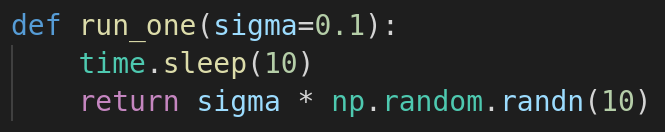
\includegraphics{run_one}

        \vskip2em
        {\large You are working on a cluster to go fast, using \code{joblib}!}\\[.5em]
        \hskip2em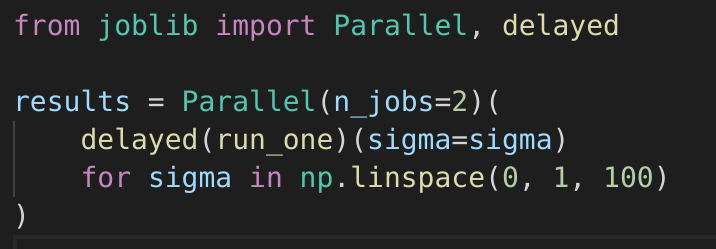
\includegraphics{parallel}
    }

        \frame{
            \frametitle{Fast computation on a cluster}
        {\large But sometime, there are unexpected crash:}\\[2em]
        \myitem{} Memory overflow
        \hskip4em\myitem{} Job preemption (SLURM)\\[1em]
        \myitem{} Unexpected reboot
        \hskip3.2em\myitem{} Pathological cases

        \vskip2em
        \strongpoint{\large You need to restart from scratch...}
    }

    \frame{
        \frametitle{Fault-tolerant computations using \code{joblib.Memory}}

        {\large {\bf Simple solution:} Use \code{joblib.Memory}:}\\[1em]
        \hskip2em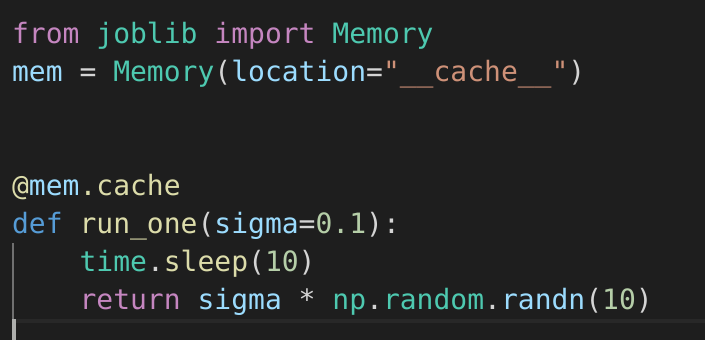
\includegraphics{memory.png}

    }
    \frame{
        \frametitle{Fault-tolerant computations using \code{joblib.Memory}}

        \centering
        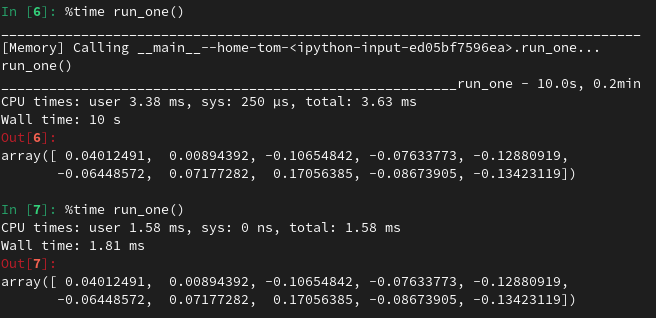
\includegraphics[width=.9\textwidth]{time_run_one}

        \pause
        \strongpoint{Be careful with randomness!}
    }

    \frame{
        \frametitle{Fault-tolerant computations using \code{joblib.Memory}}


        {\large {\bf Caching:} ``Save'' the results of each call to \code{run\_one}}\\[2em]
        \begin{itemize}\itemsep2em
            \item Save on disk so the results persist after reboot.\\[.5em]
            \hskip5em{$\Rightarrow$ Create a file with the result.}
            \item Don't recompute if the result already exists.\\[.5em]
            \hskip5em{$\Rightarrow$ Unique id for \code{run\_one, sigma} (\emph{hash}).}
        \end{itemize}
    }

    \frame{
        \frametitle{Common pitfall: argument hashing}

        {\bf Cache Miss:}\\[.5em]
        \myitem{} Parameters you pass must be exactly the same.\\
            {\color{black!70}\hskip4em{} No approximation.}\\[.5em]
        \myitem{} Parameters need to be consistently picklable.\\
            {\color{black!70}\hskip4em{} \emph{i.e.} \code{torch.Tensor}.}\\[.5em]
        {\bf Performance drop:}\\[.5em]
        \myitem{} Hashing complex parameters can be long:\\
        {\color{black!70}\hskip4em{} \emph{i.e.} nested \code{dict}.}\\


        \vskip2em
        {\hskip2em {\bf Advice:} pass simple argument, load data in \code{run\_one} if possible.\\}
    }
    \frame{
        \frametitle{Some more info}

        {\bf Automatic cache clean:}\\[.5em]
        \myitem{} If \code{run\_one} changes, the cache is automatically erased\\[.5em]
            {\color{black!70}\hskip4em{} Changes in global variables can affect it.}\\[1em]

        {\bf Ignore parameters:}\\[.5em]
        \myitem{} You can ignore parameters that do not change the output\\[.5em]
            {\color{black!70}\hskip4em{} \raisebox{-4em}{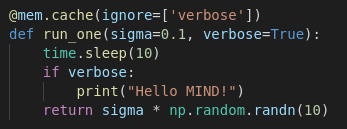
\includegraphics[height=6em]{ignore}}}\\
    }

\end{document}